\subsection{Implementation}
Bevor die in \autoref{sec:wireframes} entwickelten Konzepte realisiert werden, muss das Projekt in der Godot Engine konfiguriert werden.
Im Anschluss werden Kernmechaniken, wie Bewegung des Charakters oder des Partners, realisiert.
Auf diesen Grundlagen können dann die ermittelten Hypothesen implementiert werden.
Dieser Vorgang wird in diesem Abschnitt beschrieben.
Das Spiel trägt den Titel \texttt{EvoWorld} und ist als 2D-Pixel-Art-Spiel ausgearbeitet.

\subsubsection{Konfiguration}
Aufgrund der Tatsache, dass es sich um ein Spiel in Pixel-Grafik handelt, ist die Fenstergröße dementsprechend konfiguriert.
In der Projekteinstellungen der Godot Engine ist die Größe auf 320x180 eingestellt.
Diese wird später künstlich auf 1280x720 hochskaliert.
Ebenfalls müssen Einstellungen in dem Physik-Modul vorgenommen werden.
Das Kollisionsystem der Godot Engine basiert auf einem Schichtsystem\cite{godot-collision}.
Das bedeutet, dass ausgewählt werden kann, auf welcher Kollisionsebene sich ein CollisionObject2D befindet.
Der \texttt{Layer} gibt an, auf welcher Ebene sich das Objekt befindet und eine \texttt{Mask} gibt an, mit welcher Ebene dieses kollidieren kann.
Im Projekt sind vier verschiedene Ebenen spezifiziert.\\

Die World-Ebene gibt an, welche Kollisionsobjekte sich in der Welt befinden.
Ein Beispiel dafür sind Wände, welche nicht von Spielenden, Gegnern oder \ac{NPC} passierbar sind.
Drei weitere Ebenen sind die Player-, Enemy- und \ac{NPC}-Ebene.
Die Player-Ebene ist nötig, um bestimmte Funktionen auszulösen.
Beispielhaft wäre eine Kollision des Hauptcharakters auf der Player-Ebene mit einem Gegner auf der Enemy-Ebene.
Dies resultiert in einem Kampf.
Die \ac{NPC}-Ebene wird dafür verwendet, dem Hauptcharakter eine Interaktion mit den \ac{NPC} zu ermöglichen.

\subsubsection{Assets}
Assets sind nicht-technische Inhalte, welche in Videospielen verwendet werden.
Diese können in Form von Sprites, Animationen oder Musik existieren.
Ebenfalls lassen sich noch weitere Elemente unter diesem Oberbegriff kategorisieren.
Der Fokus lag in der Arbeit allerdings auf visuellen Assets in Form von Sprites.
Für diesen Zweck entstand eine interdisziplinäre Kooperation mit einer Game Art \& 3D Animation Studentin des SAE Instituts\cite{sae-institute}.
Diese Kooperation ist aufgrund zeitlicher Probleme pausiert und kann erst nach der Arbeit fortgesetzt werden.
Zwei Assets sind innerhalb dieser Kooperation entstanden.
Das Sprite des Hauptcharakters und eines Gegners.
Alle weiteren Sprites sind selbst entwickelt.
Lediglich die Schriftart \texttt{NESCyrillic} ist noch ein weiteres externes Asset.
Alle Lizenzen und Referenzen zu den Inhalten sind in der \texttt{README.md} des Projekts angegeben.

\subsubsection{Bewegung}
Eine wichtige Kernmechanik eines Rollenspiels ist die Bewegung des Charakters.
Die Bewegung erfolgt anhand der \texttt{WASD}-Tasten.
Die Eingabe wird als zweidimensionaler Vektor interpretiert.
Je nach Taste wird der X- oder Y-Wert um eins addiert oder subtrahiert.
Die Interpretation wird dann auf den Charakter angewandt, welcher sich dann in Geschwindkeit und Richtung des Vektors bewegt.
Beim Drücken der Taste \texttt{D} entsteht der Vektor $(1, 0)$ und die Länge des Vektors beträgt eins.
Dieser Vektor ist als $\vec{v}$ in \autoref{fig:distance} gekennzeichnet.\\

% 0,0 URSPRUNG
\begin{figure}[ht]
    \centering
    \scalebox{1.5}{
        \begin{tikzpicture}
            \tkzInit[xmax=1,ymax=1]
            \tkzDefPoint (1,0){A}
            \tkzDefPoint (1,1){B}
            \tkzDefPoint (0,1){C}
            \tkzDrawXY
            \tkzGrid
            \draw [red,thick,opacity=0.7, domain=0:90] plot ({cos(\x)}, {sin(\x)});
            \tkzLabelPoint[blue,above right](A){$(1,0)$}
            \tkzLabelPoint[blue, above right](B){$(1,1)$}
            \tkzDrawPoints[blue](A, B)
            \draw[line width=1pt, black, -stealth](0, 0) -- (1,1) node[midway, above]{$\vec{u}$};
            \draw[line width=1pt, black, -stealth](0, 0) -- (1,0) node[midway, below]{$\vec{v}$};
        \end{tikzpicture}
    }
    \caption{Distanz und Einheitskreis}
    \label{fig:distance}
\end{figure}

Diese Methodik birgt allerdings ein Problem.
Wenn die spielende Person zwei Eingaben auf unterschiedlichen Achsen tätigt, kann es dazu kommen, dass die Länge des Vektors nicht gleich eins beträgt.
Das liegt daran, dass die Länge eines Vektors als folgende Funktion gegeben ist\cite[S.16]{vector-math}.

\setcounter{equation}{0}
\begin{equation}
    |\vec{a}| = |\left(\begin{array}{c} a_1 \\ a_2 \end{array}\right)| = \sqrt{a_1^2 + a_2^2}
\end{equation}

Wenn eine Person nun zusätzlich zu der Taste \texttt{D} die Taste \texttt{S} betätigt, entsteht der Vektor $(1, 1)$.
Wie in der \autoref{fig:distance} zu sehen, ist die Länge des Vektors $\vec{u}$ größer als die des Vektors $\vec{v}$.
Die Länge von $\vec{u}$ beträgt nämlich $\sqrt{2}$.
Das bedeutet, dass eine Bewegung in der Diagonale schneller wäre, als eine Bewegung entlang einer der beiden Achsen.
Das Problem kann allerdings umgangen werden, wenn dieser Vektor normiert wird\cite[S.22]{vector-math}.
Dies sorgt dafür, dass der Vektor auf die Länge des Radius vom Einheitskreises reduziert wird, welcher in rot eingezeichnet ist.
Dieser Radius beträgt eins.\\

Damit der Charakter langsam beschleunigt, wird die \texttt{move\_toward}-Funktion verwendet\cite{godot-move-toward}.
Diese erhöht oder verringert einen Vektor bezüglich eines anderen Vektors in Abhängigkeit von \texttt{delta}.
Ebenfalls wird diese Funktion verwendet, um den Charakter bei keiner Eingabe langsam auzubremsen.
Die \texttt{move\_and\_slide}-Funktion sorgt dann dafür, dass sich dieser in Richtung des Vektors bewegt\cite{godot-move-and-slide}.
Falls der Charakter mit einer CollisionShape2D kollidiert, stoppt dieser nicht, sondern gleitet an der Form der CollisionShape2D entlang.\\

Ein RayCast2D gibt die Rotation des Charakters an.
Diese wird mithilfe der Funktion \texttt{atan2} und dem Eingabevektor als Übergabeparameter berechnet\cite{godot-builtins}.
Das Resultat ist der Polarwinkel $\varphi$, welcher die aktuelle Rotation in Radiant angibt.\\

\subsubsection{Menüs}
Im Rahmen des Projekts sind mehrere Menüs und ein Pop-up entwickelt worden.
Das Startmenü ermöglicht es, den Spielenden auszuwählen, ob diese mit dem Spiel beginnen möchten oder zunächst Einstellungen vornehmen wollen.
Es existiert zwar ein Einstellungsmenü, allerdings ist dieses nicht technisch implementiert.
Das liegt daran, dass der Fokus zunächst auf das Gameplay gelegt ist.
Das erwähnte Pop-up ist das Fenster, welches angezeigt wird, wenn die spielende Person einen Kampf verliert und ihr die verlorenen Gegenstände mitgeteilt werden sollen. \\

\begin{figure}[H]
    \centering
    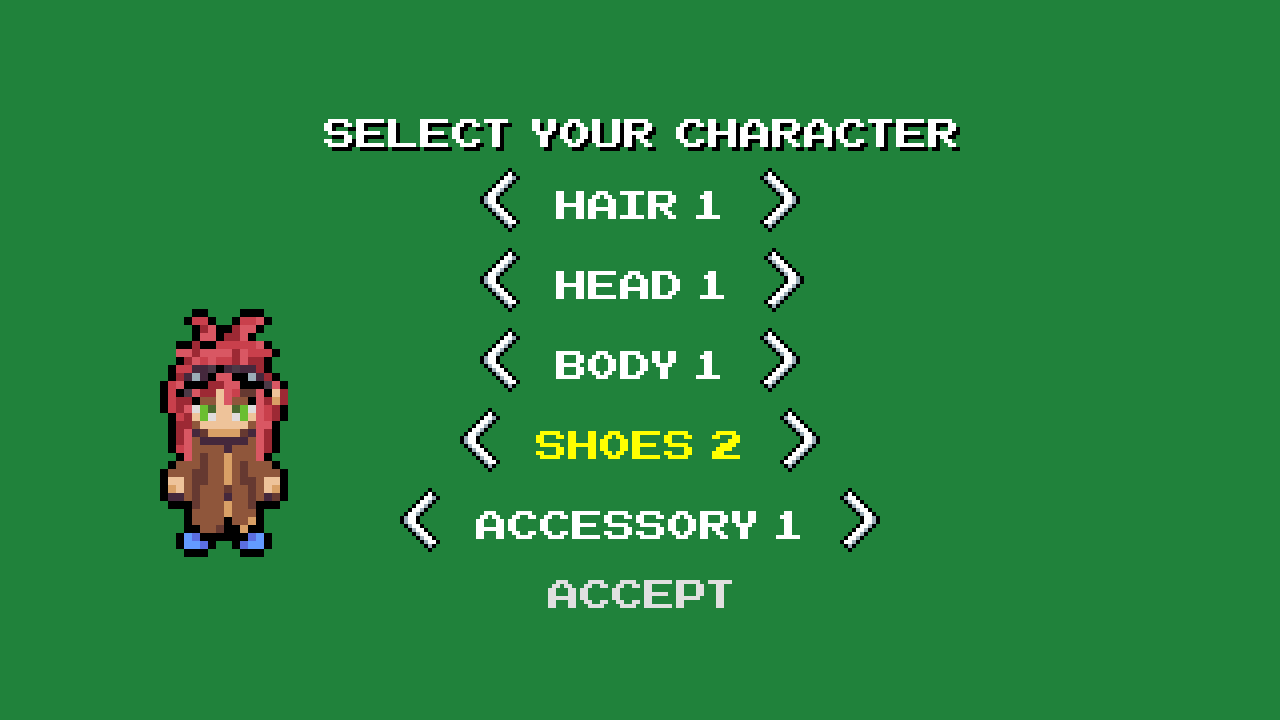
\includegraphics[width=0.8\columnwidth]{figures/screenshots/charselect.png}
    \caption{\label{fig:char-impl}Charakterauswahlmenü}
\end{figure}

Wenn die spielende Person das Spiel beginnt, landet diese zunächst im Charakterauswahlmenü.
Dieses Menü ist in \autoref{fig:char-impl} dargestellt und nach dem in \autoref{sec:wireframes} vorgestellten Wireframe modelliert.
Die Szene ist primär mithilfe von Control-Nodes aufgebaut.
Allerdings befindet sich innerhalb dieser Control-Nodes die Node des Hauptcharakters.
Diese ist zusammengesetzt aus verschiedenen Sprite-Nodes, welche die einzelnen Körperteile repräsentieren.
Beim Wechsel der einzelnen Komponenten wird die Funktion \texttt{\_on\_button\_pressed} im Skript des Menüs ausgelöst.
Dies sorgt dafür, dass die Zahl hinter der Bezeichnung eines Elements angepasst und die Informationen über die aktuelle Auswahl dem \texttt{Player}-Node übergeben wird.
Dort werden die entsprechenden Sprites angezeigt, welche bereits vom Skript \texttt{sprites.gd} mithilfe von \texttt{preload} vorgeladen sind.
In Hinblick auf die weitere Entwicklung nach dieser Arbeit werden diese Daten ebenfalls in einem Autoload-Skript gespeichert.
Diese können dann an unterschiedlichen Orten geladen werden, um die \texttt{Player}-Node mit den zuvor gespeicherten Sprites zu laden.
Nach Betätigen des \texttt{Accept}-Knopfes landet die spielende Person im Spiel. \\

\begin{figure}[H]
    \centering
    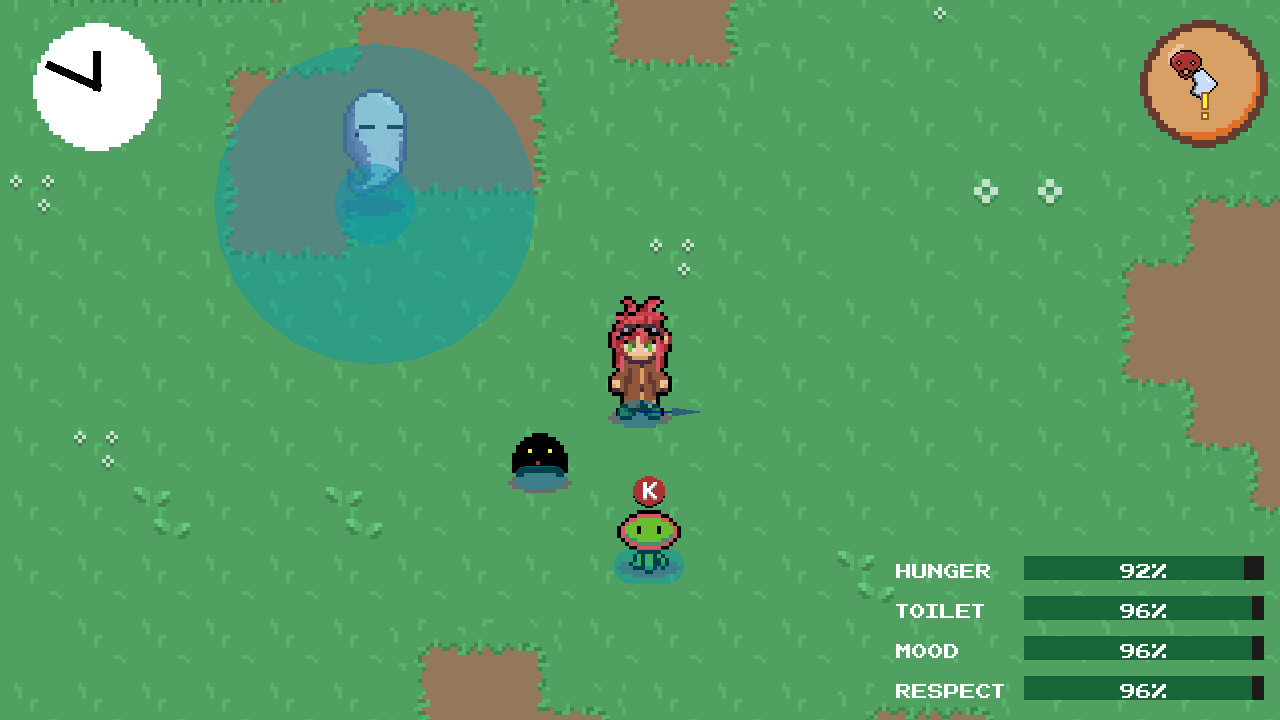
\includegraphics[width=0.8\columnwidth]{figures/screenshots/ingame.png}
    \caption{\label{fig:ingame}Innerhalb der Spielwelt}
\end{figure}

\autoref{fig:ingame} zeigt den Spielinhalt, wenn eine spielende Person den Charakter ausgewählt hat.
Diese Abbildung enthält mehrere Informationen, welche im Folgenden erklärt werden.
Die blauen Kreise um einzelne Objekte sind CollisionShapes, welche aktiviert sind, um die Inhalte des Spiels besser erklären zu können.
Als Erstes wird das \ac{HUD} näher beschrieben.
Dieses ähnelt dem \ac{HUD} in Digimon World, mit dem Zusatz, dass eine Minimap und weitere Fortschrittsbalken existieren.
Ebenfalls ist die Uhr als 12-Stunden-Anzeige mit zwei Zeigern modelliert.\\

Die Karte ist anhand eines Tutorials implementiert\cite{kids-minimap}.
Dieses Tutorial ist verwendet worden, weil es dem Entwurf in \autoref{sec:wireframes} entspricht.
Jedes Objekt, welches in der Minimap vorkommt, besitzt die Variable \texttt{minimap\_icon}, welche dafür zuständig ist, das Objekt mit dem korrekten Symbol auf der Karte einzublenden.
Alle Nodes, welche diese Eigenschaft besitzen, werden der Gruppe \texttt{minimap\_objects} zugeordnet.
\autoref{lst:group} zeigt die Möglichkeit, mithilfe von Gruppen alle Nodes zu filtern, welche sich in der Gruppe \texttt{minimap\_objects} befinden und im Szenengraph vorhanden sind.\\

\begin{listing}[H]
    \caption{Nodes innerhalb einer Gruppe}
    \label{lst:group}
    \begin{minted}
[
bgcolor=LightGray,
framesep=2mm,
baselinestretch=1.2,
fontsize=\footnotesize,
linenos,
]{gd.py:GDScriptLexer -x}
var map_objects = get_tree().get_nodes_in_group("minimap_objects")
\end{minted}
\end{listing}

Eine neue Aufgabe besitzt den Wert \texttt{quest} und ist als gelbes Ausrufezeichen modelliert.
Gegner besitzen den Wert \texttt{enemy} und sind als rote Totenkopfschädel modelliert.
Objekte außerhalb des sichtbares Bereiches werden am Rande der Karte verkleinert dargestellt.
Ebenfalls ist es möglich, mithilfe des Mausrads das Zoomlevel der Karte einzustellen. \\

\begin{figure}[H]%
    \centering
    \subfloat[\centering Aufgabenliste]{{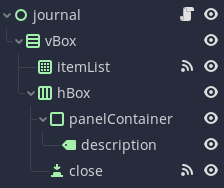
\includegraphics[width=5cm]{figures/screenshots/journal.png} }\label{fig:journal-a}}%
    \qquad
    \subfloat[\centering Inventar]{{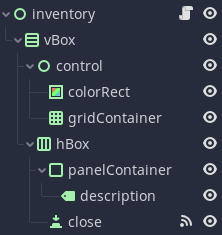
\includegraphics[width=5cm]{figures/screenshots/inventory.png}
                \label{fig:inventory-b}}}%
    \caption{Aufgabenliste und Inventar}%
    \label{fig:inventory-journal-impl}%
\end{figure}

\autoref{fig:inventory-journal-impl} verdeutlicht den Szenengraphen der Aufgabenliste und des Inventars.
Die Beschreibung und der \texttt{Schließen}-Knopf haben in beiden Fällen dieselbe Funktionalität.
Die Beschreibung gibt Details über eine Aufgabe oder einen Gegenstand an, welcher aktuell selektiert ist.
Mithilfe eines Signals des Knopfes wird das Event \texttt{close\_button\_pressed} gefeuert, welches dafür sorgt, dass ein aktives Fenster geschlossen wird. \\

Die Aufgabenliste in \autoref{fig:journal-a} ist anhand einer ItemList implementiert\cite{godot-itemlist}.
Diese beinhaltet eine Spalte, der Elemente hinzugefügt werden können.
Falls die Liste zu viele Elemente enthält, um alle darzustellen, wird eine Scrollleiste hinzugefügt.
Die ItemList besitzt das Signal \texttt{item\_selected}, welches gefeuert wird, wenn ein Element in der Liste ausgewählt wird.
Innerhalb des Skripts \texttt{journal.gd} wird die Beschreibung dann durch die Beschreibung des jeweiligen Elements ersetzt.\\

Das Inventar hingegen ist mit einem GridContainer konstruiert worden\cite{godot-gridcontainer}.
Dies ist in \autoref{fig:inventory-b} zu sehen.
Der GridContainer besitzt eine feste Anzahl von Reihen und Spalten.
Ebenfalls ist der Hintergrund durchsichtig.
Aus diesem Grund wird ein ColorRect verwendet, um die Hintergrundfarbe zu definieren\cite{godot-colorrect}.
Die feste Anzahl wurde hier verwendet, um den Platz des Inventars zu begrenzen.
Die einzelnen Aufgaben oder Gegenstände sind ebenfalls in Hinblick auf die Zukunft innerhalb der \texttt{PlayerVariables} gespeichert.\\

Die Statuswerte des Partners, welche in \autoref{fig:ingame} dargestellt sind, werden durch Prozentzahlen repräsentiert.
Dies soll helfen, die aktuelle Lage besser einschätzen zu können, statt diese Werte nur anhand der Fortschrittsbalken abzuschätzen.
Ebenfalls besitzt jeder Fortschrittbalkens ein Label, welches diesen beschreibt.
Die Werte werden aktuell mithilfe eines Timers und nach einem bestimmten Intervall weniger.
Diese Änderung wird dann mithilfe des Signals \texttt{status\_changed} über den Eventbus gefeuert. \\

\subsubsection{Non-player character}\label{sec:npc}
Die in \autoref{fig:ingame} abgebildete Blume ist ein ansprechbarer \ac{NPC}.
Dieser besitzt eine \texttt{triggerZone}, welche ein Signal feuert, wenn die spielende Person diese betritt.
Die Auswirkung davon ist, dass der Interaktionsknopf über dem Sprite des \ac{NPC} zu sehen ist. \\

\begin{listing}[H]
    \caption{RayCast Interaktion mit einem \ac{NPC}}
    \label{lst:handle-colliding}
    \begin{minted}
[
bgcolor=LightGray,
framesep=2mm,
baselinestretch=1.2,
fontsize=\footnotesize,
linenos,
]{gd.py:GDScriptLexer -x}
func _handle_colliding() -> void:
	if !Input.is_action_just_pressed("confirm"):
		return
		
	if !ray.is_colliding():
		return
	
	var target = ray.get_collider().get_parent()
	EventBus.emit_signal("confirm_button_pressed", target)
\end{minted}
\end{listing}

\autoref{lst:handle-colliding} beschreibt die technische Umsetzung, um mit diesem \ac{NPC} zu interagieren.
Zunächst muss die spielende Person die Taste \texttt{K} betätigen.
Ebenfalls muss der RayCast2D mit einem \ac{NPC} kollidieren.
Das bedeutet, dass die spielende Person sehr nah stehen und in die Richtung des \ac{NPC} schauen muss.
Hierfür wurden Kollisionsmasken verwendet, um sicherzustellen, dass nur interagierbare Objekte mit dem RayCast2D kollidieren können.
Falls beide Konditionen erfüllt sind, wird das interagierbare Objekt über den Eventbus als Signal verschickt.
Jede \ac{NPC}-Node hört auf dieses Signal und validiert, ob \texttt{target} mit der Node übereinstimmt.
Falls dies der Fall ist, wird ein Dialog gestartet.

\subsubsection{Dialoge}
Dialoge sind mithilfe der Erweiterung Dialogic umgesetzt\cite{github-dialogic}.
Diese Erweiterung fügt einen weiteren Reiter mit dem gleichen Namen im Editor hinzu.
In dieser Komponente können Dialoge entsprechend konfiguriert werden.
Beispielhaft wird der Dialog mit der in \autoref{sec:npc} erwähnten Blume näher erläutert.\\

\begin{figure}[H]
    \centering
    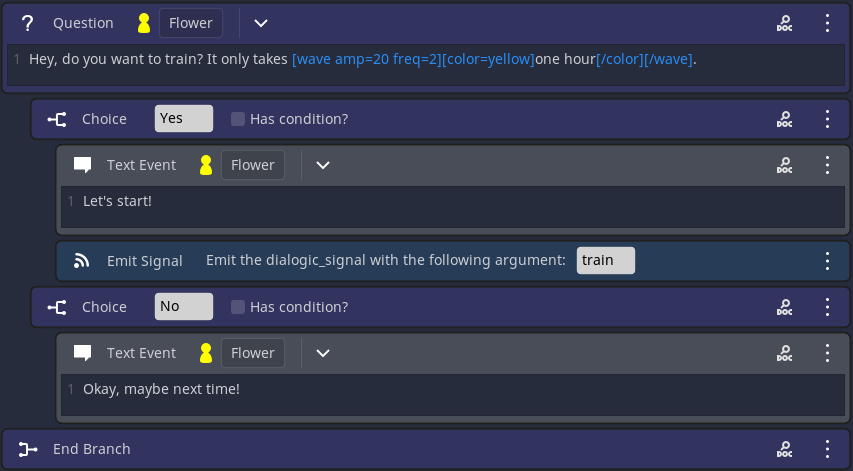
\includegraphics[width=0.9\columnwidth]{figures/screenshots/dialogic.png}
    \caption{\label{fig:dialogic}Dialog mit dem \ac{NPC} Flower}
\end{figure}

Der in \autoref{fig:dialogic} dargestellte Dialog wird in Dialogic mithilfe einer Timeline umgesetzt.
Eine Timeline ist eine Abfolge von Events. Diese können Texte, bestimmte Konditionen, Signale oder weitere Events beinhalten.
In diesem Beispiel wird zunächst eine Frage gestellt, auf welche die spielende Person mit \texttt{Ja} oder \texttt{Nein} antworten kann.
Für den Fall, dass die Option \texttt{Ja} gewählt wird, wird das Signal \texttt{train} gefeuert, welches dafür sorgt, dass eine Stunde im Spiel vergeht.
Für den Fall, dass die Option \texttt{Nein} gewählt wird, passiert nichts.
In beiden Fällen wird nach auflösen der Events die Konversation beendet.
Die Texte können mithilfe von BBCode modifiziert werden.
Dies ist im ersten Event in der Abbildung zu sehen.
Dort wird eine Animation und eine farbliche Kennzeichnung für einen bestimmten Abschnitt im Text angewandt.

\subsubsection{Bewegung des Partners}
Im Referenzspiel Digimon World folgt das Partner-Digimon dem Spieler automatisch.
In der in dieser Arbeit implementierten Variante ist dies ebenfalls der Fall.
Die Bewegung des Partners zur spielenden Person erfolgt anhand linearer Interpolation.
Lineare Interpolation beschreibt in diesem Fall den Wechsel zwischen zwei Positionen $P$ und $S$.
Der Parameter $i$  gibt dabei die aktuelle Interpolation an, wobei $i$ zwischen Null und Eins liegt.
Wenn $i=0{,}5$ beträgt, befindet sich die aktuelle Position in der Mitte zwischen $P$ und $S$.
Mithilfe der, von der Godot Engine bereitgestellten, Funktion \texttt{linear\_interpolate} kann die beschrieben Interpolation umgesetzt werden.
Dafür wird als Zielposition die Position des Hauptcharakters gewählt und die Interpolation errechnet sich aus \texttt{delta} multipliziert einer konstanten Geschwindigkeit. \\

\subsubsection{Bewegung des Gegners}
Die Bewegungsmuster des Gegners sind mithilfe eines endlichen Automaten realisiert.
\autoref{fig:fsm} zeigt alle möglichen Zustände an, welche ein Gegner annehmen kann.
Die Zustandswechsel erfolgen unter drei verschiedenen Bedingungen.
Der Hauptcharakter hat die in \autoref{fig:ingame}, um den Gegner markierte, \texttt{triggerZone} betreten oder verlassen, eine bestimmte Distanz zu einem Zielpunkt ist erreicht oder ein Timer ist abgelaufen.
Der Zustand \texttt{WANDER} ($w$) ist als Initalzustand festgelegt.
In diesem Zustand bewegt sich der Gegner auf einen zufällig ausgewählten Zielpunkt innerhalb eines bestimmten Radiuses zu.
Wenn dieser eine bestimmte Distanz zum Zielpunkt erreicht oder das Signal des Timers \texttt{\_on\_timer\_timeout} feuert, wechselt der Zustand in den \texttt{STOP}-Zustand ($s$).
Direkt zurück in den Zustand $w$ kommt der Gegner nur, wenn das Signal des Timers erneut gefeuert wird.
Dieses Verhalten soll einen Gegner simulieren, welcher in einem bestimmten Radius umherwandert. \\

\tikzset{
->,
node distance=3cm, .
every state/.style={thick, fill=gray!10},
initial text=$ $,
}


\begin{figure}[H]
    \centering
    \begin{tikzpicture}
        \node[state, initial] (w) {$w$};
        \node[state, right of=w] (s) {$s$};
        \node[state, below of=w] (m) {$m$};
        \node[state, right of=m] (c) {$c$};
        \node[state, accepting, right of=c] (f) {$f$};
        \draw (w) edge[right] node{trigger} (c);
        \draw (c) edge[above, bend right] node{trigger} (m);
        \draw (m) edge[above, bend right] node{trigger} (c);
        \draw (m) edge[left] node{distance} (w);
        \draw (w) edge[above] node{distance} (s);
        \draw (w) edge[above, bend left] node{timer} (s);
        \draw (s) edge[above, bend left] node{timer} (w);
        \draw (s) edge[right] node{trigger} (c);
        \draw (c) edge[above] node{fight} (f);
    \end{tikzpicture}
    \caption{Nichtdeterministischer endlicher Automat}
    \label{fig:fsm}
\end{figure}

Beide Zustände können mithilfe des Signals \texttt{\_on\_triggerZone\_player\_entered} der \texttt{triggerZone} in den Zustand \texttt{CHASE\_PLAYER} ($c$) wechseln.
Wenn der Gegner in diesem Zustand ist, bewegt er sich auf den Hauptcharakter zu.
Sollte es zu einer Kollision mit dem \texttt{fightTrigger} kommen, wird das Signal \texttt{combat\_started} über den Eventbus gefeuert.
Anschließend findet ein Kampf statt und der Automat erreicht den Endzustand $f$.
Für den Fall, dass die Distanz zum Hauptcharakter größer als ein festgelegter Wert ist, wird der Zustand auf \texttt{MOVE\_BACK} ($m$) gesetzt.
Dabei wird erneut das Signal \texttt{\_on\_triggerZone\_player\_entered} gefeuert.
In diesem Fall ist der Wert des Signals allerdings \texttt{false}.
Im Zustand ($m$) bewegt sich der Gegner zur Startposition zurück.
Sollte die Spielende Person die \texttt{triggerZone} erneut auslösen, verfolgt der Gegner den Hauptcharakter erneut.
Wenn allerdings die Startposition erreicht wird, wandert der Gegner erneut umher.\\

\subsubsection{Kampf}
\autoref{fig:combat} stellt eine Kampfsituation dar.
Diese ist nach dem Entwurf in \autoref{fig:battle-wireframe} modelliert.
Sie besitzt allerdings einige technische Besonderheiten, welche in diesem Abschnitt erklärt werden.

\begin{figure}[H]
    \centering
    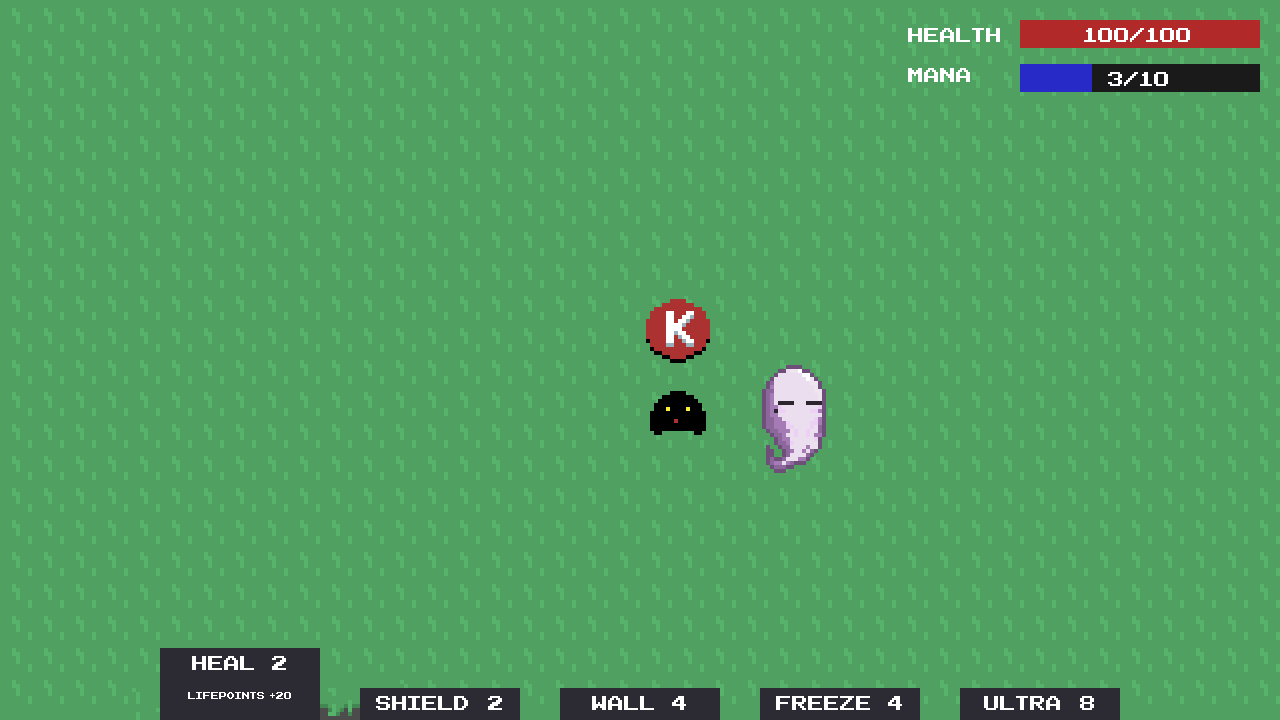
\includegraphics[width=0.8\columnwidth]{figures/screenshots/combat.png}
    \caption{\label{fig:combat}Kampfszene}
\end{figure}

Zunächst sind die Szenengraphen für \texttt{Pet} und \texttt{Enemy} als eine neue Szene abgebildet.
Die Szene \texttt{CombatEntity}, welche als Ersatz für beide Entitäten dient, wird an dieser Stelle verwendet, um den Entwicklungsprozess zu beschleunigen.
Das liegt daran, dass ansonsten Werte zwischengespeichert und in eine neue Szene übertragen werden müssten.
Ebenfalls müsste das Skript für beide Nodes stark angepasst werden.
Der Unterschied zwischen den beiden Entitäten wird im Skript mithilfe eines Booleans repräsentiert.
Das bedeutet, dass einige Zeilen Code nur für das \texttt{Pet} ausgeführt werden.\\

In einem Kampf bewegen sich beide Entitäten aufeinander zu.
Dies geschieht mithilfe den vorher erwähnten Funktionen \texttt{move\_towards} und \texttt{move\_and\_slide}.
Wenn eine gewisse Distanz zwischen beiden Entitäten erreicht ist, wird die Zeit mithilfe des Parameters \texttt{time\_scale} des \texttt{Engine}-Singletons heruntergesetzt\cite{godot-class-engine}.
Das Resultat ist, dass die Zeit im Spiel langsamer verläuft.
Danach wird ein Timer gestartet, welcher die Zeit wieder zurücksetzt.
Während dieser Timer läuft, wird der spielenden Person die Taste \texttt{K} angezeigt, welche geklickt werden kann, um Mana im Kampf zu generieren. \\

Aufgrund der Tatsache, dass beide Entitäten aufeinander zulaufen, kommt es ab einem gewissen Zeitpunkt zu einem Kontakt.
Wenn beide Entitäten kollidieren, wird der Schaden berechnet und ein Rückstoß ausgeführt.
Der Rückstoß wird als Vektor repräsentiert und auf die aktuelle Geschwindigkeit addiert.
Das Problem mit dieser Mechanik ist, dass beide Entitäten in dieselbe Richtung gestoßen werden können und die Methode \texttt{\_on\_area2D\_area\_entered} nicht erneut ausgeführt wird, weil die Area2D nie verlassen wurde.
Das sorgt dafür, dass kein neuer Rückstoß berechnet wird und beide Entitäten sich nicht mehr bewegen.
Aus diesem Grund sorgt ein Timer dafür, dass regelmäßig ein Rückstoß berechnet wird, solange beide Entitäten kollidieren.
Erst, wenn der Rückstoß dafür sorgt, dass die Kollision stoppt, stoppt auch der Timer.\\

Während die spielende Person mit der \texttt{K}-Taste im Kampf darauf aufpassen muss das korrekte Timing zu treffen, kann sie mit der \texttt{A}- und \texttt{D}-Taste durch die Karten navigieren.
Dabei wird die Karte, welche aktuell ausgewählt ist, leicht angehoben, damit die spielende Person Effektbeschreibungen lesen kann.
Ebenfalls soll dies verhindern, dass der Kampf zu stark in den Hintergrund rückt. \\

In \autoref{sec:wireframes} wurde erwähnt, dass Kampfstile, wie zum Beispiel aggressiv oder defensiv, erst in einem weiteren Schritt nach der Arbeit implementiert werden.
Diese können dann mithilfe der \texttt{Q}- und \texttt{E}-Taste ausgewählt werden.
Weil beobachtet wurde, dass Spielende allgemein den Kampfstil selten wechseln, sollte dies auch kein Problem darstellen.
Dies ist allerdings zunächst nur eine Hypothese, welche nach der Arbeit näher untersucht werden muss.
Das Kartensystem ermöglicht aktuell nur die Verwendung der Heilungskarte.
Diese kann mithilfe der \texttt{W}-Taste ausgewählt werden.
